%% \chapter[htoc-titlei][hhead-titlei]{htitlei}
%% -----------------------------------------------------------------------------
\chapter[The LHC and the \atlas\ experiment][The LHC and \atlas]
        {The Large Hadron Collider and the \atlas\ experiment}
\label{ch:lhc}

\begin{quote}
  As the name suggests, the Large Hadron Collider (LHC) is a particle collider,
  which collides particles at very high energies.
  There are four major experiments, including \atlas, which collect and study
  data generated from these particle collisions in an effort to study
  the properties of nature, and search for signs of physics beyond the Standard
  Model.
  This chapter gives a brief introduction to the LHC machine, and the
  \atlas\ experiment.
\end{quote}

%% ------------------------------------------------------------------------------
\FloatBarrier
\section{The LHC}
\label{sec:lhc}

The LHC~\cite{cern-jinst-lhc} is circular particle accelerator, with a
circumference of 27~km, built 100~m underground, underneath the French-Swiss
border near the city of Geneva, Switzerland, shown in
Figure~\ref{fig:lhc_aerial}.
The LHC is operated by the European Organization for Nuclear Research
(CERN~\footnote{Conseil Europ\'een pour la Recherche Nucl\'eaire}).
The LHC became fully operational in 2010, providing proton-proton collisions
to the experiments along the ring at an unprecedented center-of-mass energy
of 7~\TeV.
In 2012, the energy was increased to 8~\TeV.

\begin{figure}[ht]
  \centering
  \includegraphics[width=\textwidth, clip=true, trim=0 0 1cm 0]
    {figs/lhc/lhc_aerial.pdf}
  \caption{
    Areal view of the Geneva area with an overlaid drawing of the LHC
    and experiments~\cite{lhc_aerial}.
  }
  \label{fig:lhc_aerial}
\end{figure}

Four major experiments are positioned around the LHC to collect and analyze
data from the hadron collisions.
The experiments include \atlas~\cite{cern-jinst-atlas},
\cms~\cite{cern-jinst-cms}, \alice~\cite{cern-jinst-alice,}, and
\lhcb~\cite{cern-jinst-lhcb}.
\atlas\ and \cms\ are designed to be ``general purpose experiments,'' searching
for physics beyond the Standard Model which may present itself in may ways.
The two experiments complement each other by providing independent results,
which can be verified against the each other.
\alice\ is designed to study the heavy ion (lead nuclei) collisions, studying
the properties of quark-gluon plasma.
The \lhcb\ experiment is primarily interested in studying the physics of
$b$-hadrons.

%% ------------------------------------------------------------------------------
\FloatBarrier
\subsection{CERN accelerator complex}
\label{sec:accelerator_complex}

The LHC is only the final stage in a series of accelerators, operated by CERN,
used to provide high energy particle collisions.
For proton-proton collisions, protons begin in the Linac 2 linear
accelerator, where they are accelerated to an energy of 50~\MeV\ per proton.
From there, they are fed through several circular accelerators, including
the Proton Synchrotron Booster (PSB), Proton Synchrotron (PS), and the Super
Proton Synchrotron (SPS), where the protons are accelerated to energies of
1.4~\GeV, 25~\GeV, and 450~\GeV\ respectively.
At this stage, the protons are injected into the LHC accelerator, where 
in 2012, they were accelerated to an energy of 4~\TeV\ per proton, and finally
collided.
A schematic of the CERN accelerator complex, and how they link to one another
is shown in Figure~\ref{fig:cern_complex}.

\begin{figure}[ht]
  \centering
  \includegraphics[width=\textwidth, clip=true, trim=15cm 0 15cm 10cm]
    {figs/lhc/accelerator_complex.jpg}
  \caption{
    Schematic view of the CERN accelerator complex~\cite{Marcastel:1621583}.
  }
  \label{fig:cern_complex}
\end{figure}

Rather than a constant stream of protons, the protons in the LHC are separated
into over 1000 bunches, each containing over $10^{11}$ protons.
In each of the interaction points around the LHC ring, proton bunches cross
onces every 50~ns, where each crossing leads to potential collisions between
the constituent protons.
The instantaneous luminosity of collisions in these bunch crossings is given by
\begin{equation}
  \mathcal{L}_\mathrm{instantaneous} =
  \frac{N_{1}N_{2} n_b f_\mathrm{rev}}
  {4\pi \sigma_{x} \sigma_{y}}
  F,
\end{equation}
where $N_{1,2}$ are the number of protons per bunch, $n_b$ is the number of
bunches, $f_\mathrm{rev}$ is the frequency at which the protons are revolution
frequency, $\sigma_{x,y}$ is the width of the beam in the transverse directions,
and $F$ is a reduction factor, accounting for the fact that the beams cross
at an angle, rather than head-on.
As the proton beams circulate, and undergo collisions, they tend to spread out,
increasing $\sigma_{x,y}$, and reducing the instantaneous luminosity over time.
Typically, once the LHC is filled with proton beams, and accelerated to their
full energy, they are circulated for several hours before they are dumped, and
the accelerator is filled again.

%% ------------------------------------------------------------------------------
\FloatBarrier
\section{The \atlas\ experiment}

{\color{red} Brief intro to \atlas\ before getting into the details}

\begin{figure}[ht]
  \centering
  \includegraphics[width=\textwidth, clip=true, trim=0 0 0 0]
    %{figs/lhc/atlas_det.jpg}
    {figs/lhc/atlas_det_dino_1.jpg}
    % {figs/lhc/atlas_det_dino_2.jpg}
  \caption{
    The \atlas\ experiment~\cite{Pequenao:1095924}.
  }
  \label{fig:atlas_det}
\end{figure}

%% - - - - - - - - - - - - - - - - - - - - - - - - - - - - - - - - - - - - - - -
\FloatBarrier
\subsection{Inner detector} 

{\color{red} Introduce the ID and its purpose. Review tracking.}

\begin{figure}[ht]
  \centering{
    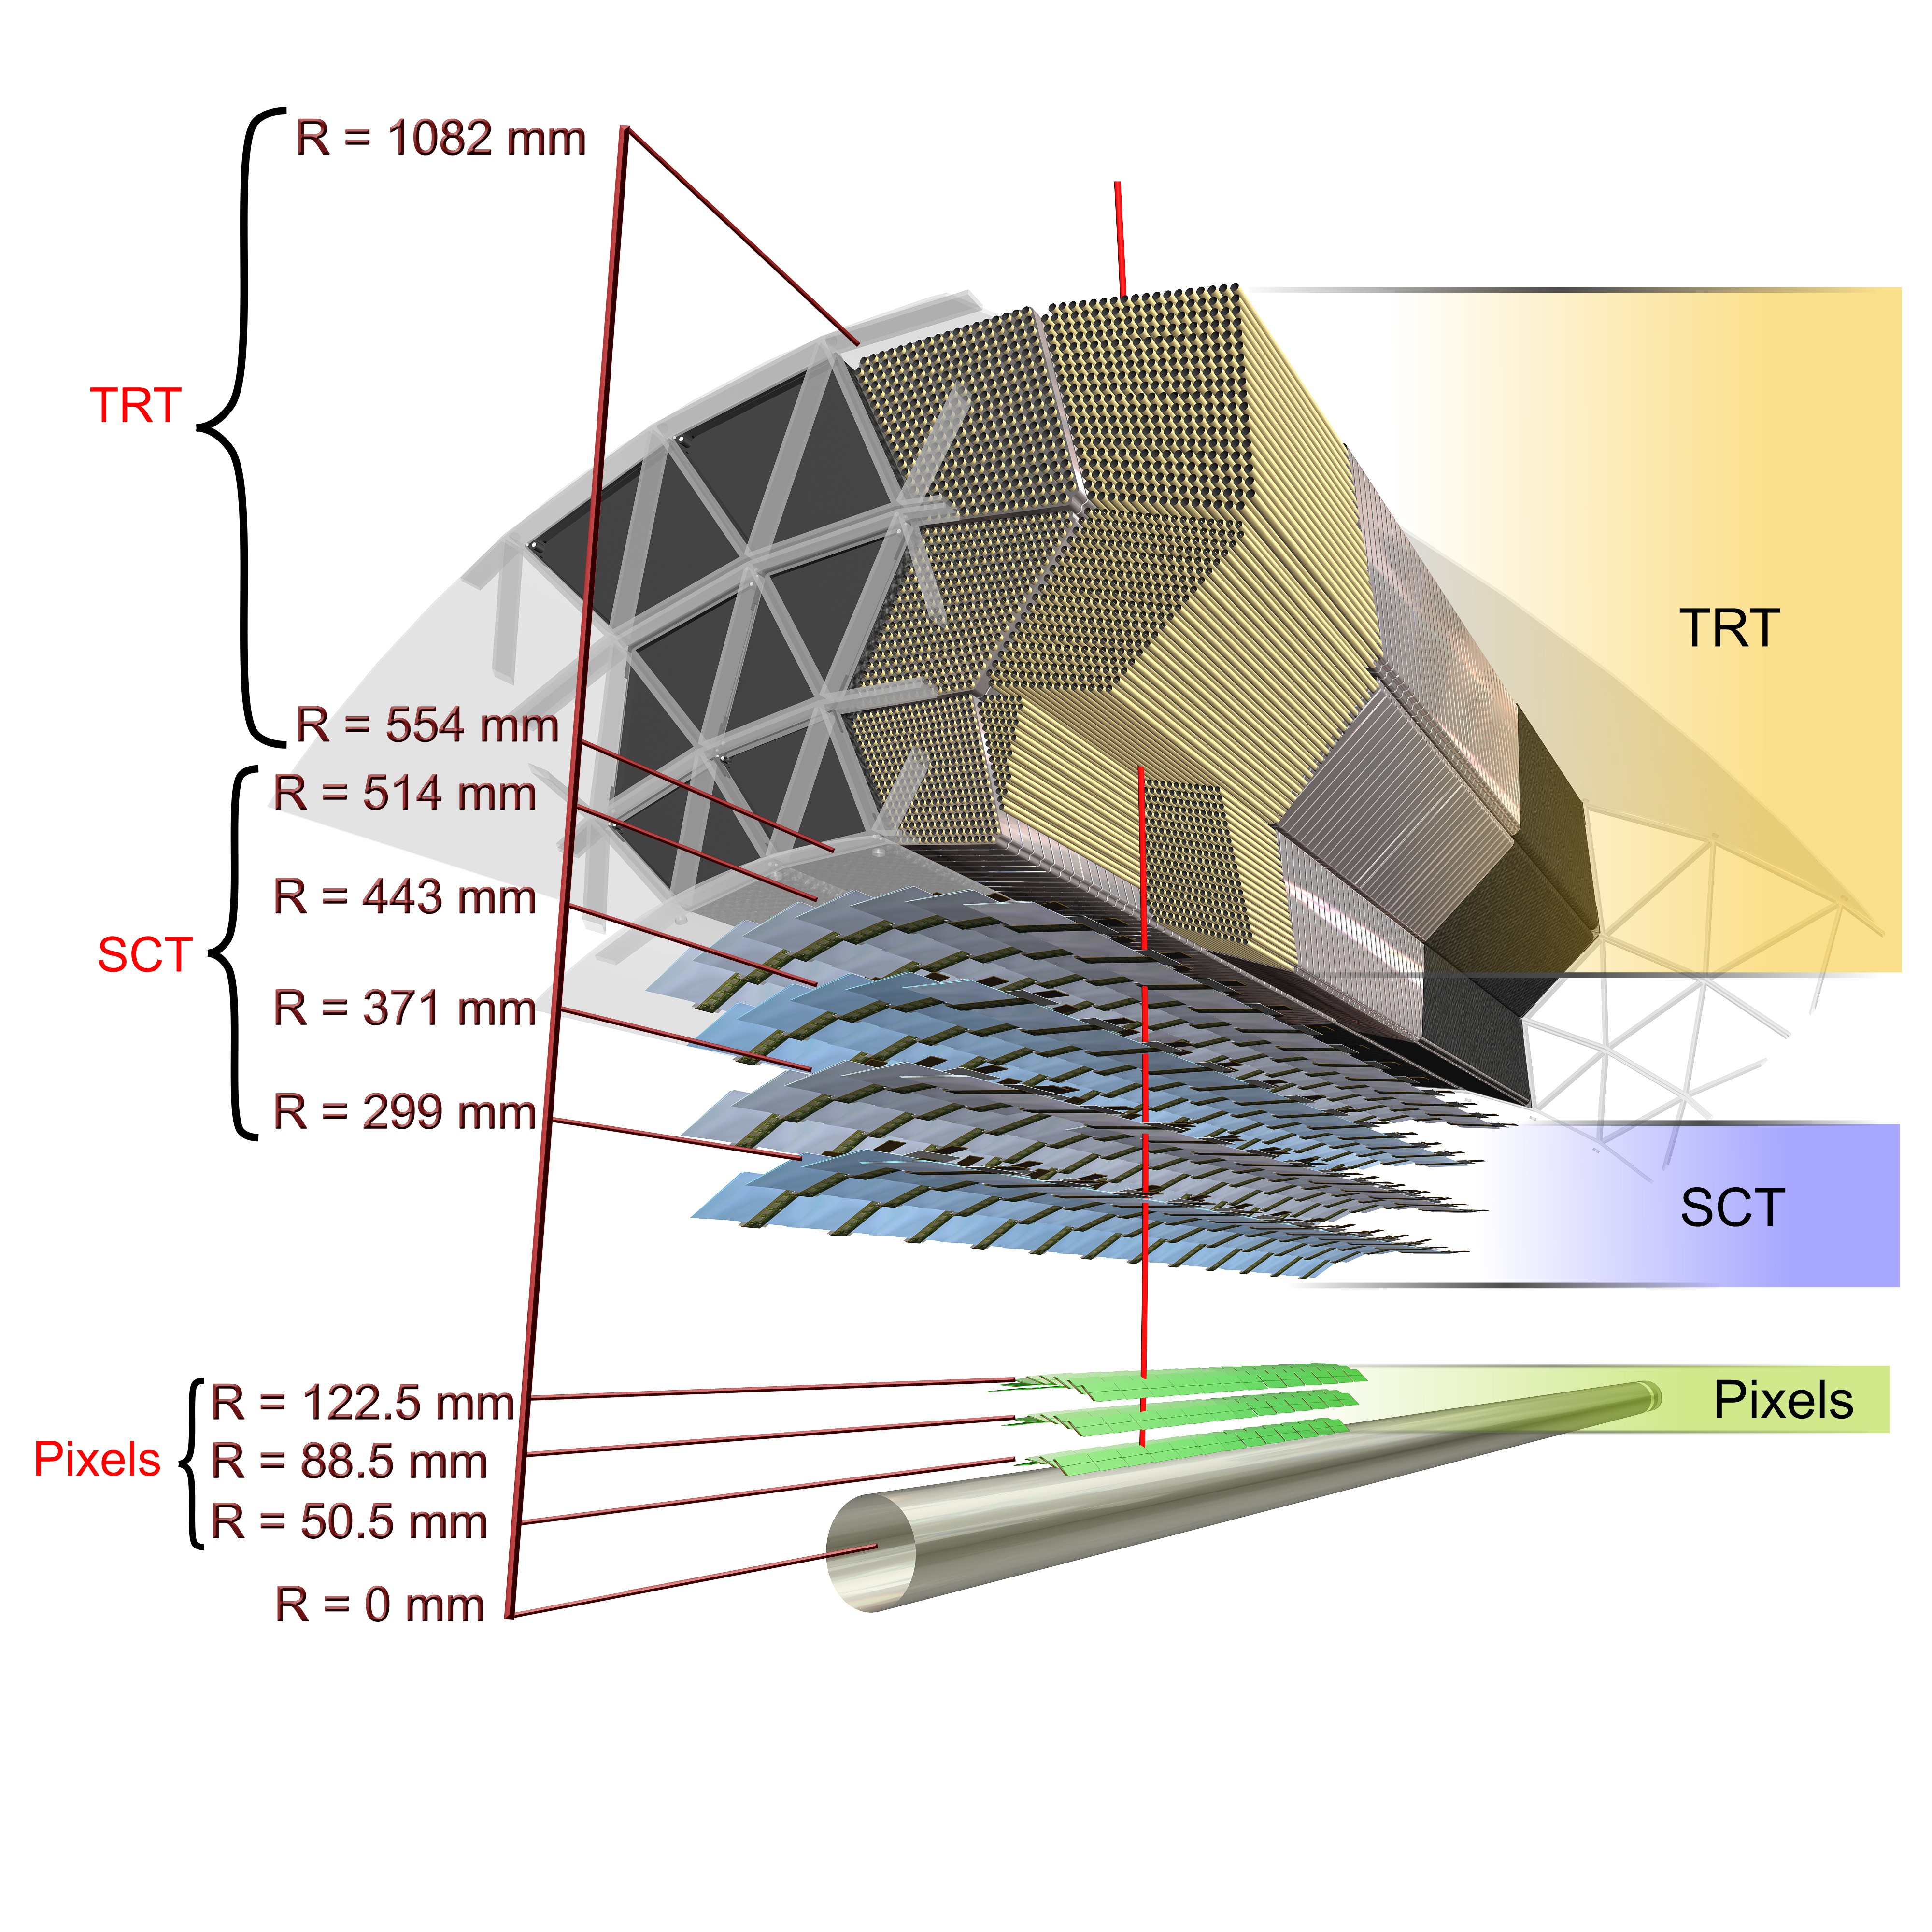
\includegraphics[width=\textwidth]{figs/lhc/id_schematic.jpg}
  }
  \caption[
    Schematic of the inner detector of the
    \atlas\ experiment~\cite{Pequenao:1095926}.
  ]{
    Schematic of the inner detector of the \atlas\ experiment.
    The inner detector is made up of layers, consisting of the silicon pixels,
    the silicon semiconductor tracker (SCT), and the transition radiation
    tracker (TRT)~\cite{Pequenao:1095926}.
  }
  \label{fig:id_cartoon}
\end{figure}

%% - - - - - - - - - - - - - - - - - - - - - - - - - - - - - - - - - - - - - - -
\FloatBarrier
\subsubsection{Pixel detector} 

\begin{figure}[ht]
  \centering{
    \includegraphics[width=\textwidth]{figs/lhc/pixel_schematic.jpg}
  }
  \caption{
    The Silicon pixel tracker of the \atlas\ experiment~\cite{Pequenao:1095925}.
  }
  \label{fig:pixel_cartoon}
\end{figure}

% \begin{figure}[ht]
%   \centering{
%     \includegraphics[width=0.8\textwidth]{figs/lhc/pixel_module.jpg}
%   }
%   \caption{{\color{red}TODO}~\cite{Wermes:43561}.}
%   \label{fig:pixel_module}
% \end{figure}

%% - - - - - - - - - - - - - - - - - - - - - - - - - - - - - - - - - - - - - - -
\FloatBarrier
\subsubsection{Silicon semiconductor tracker} 

\begin{figure}[ht]
  \centering{
    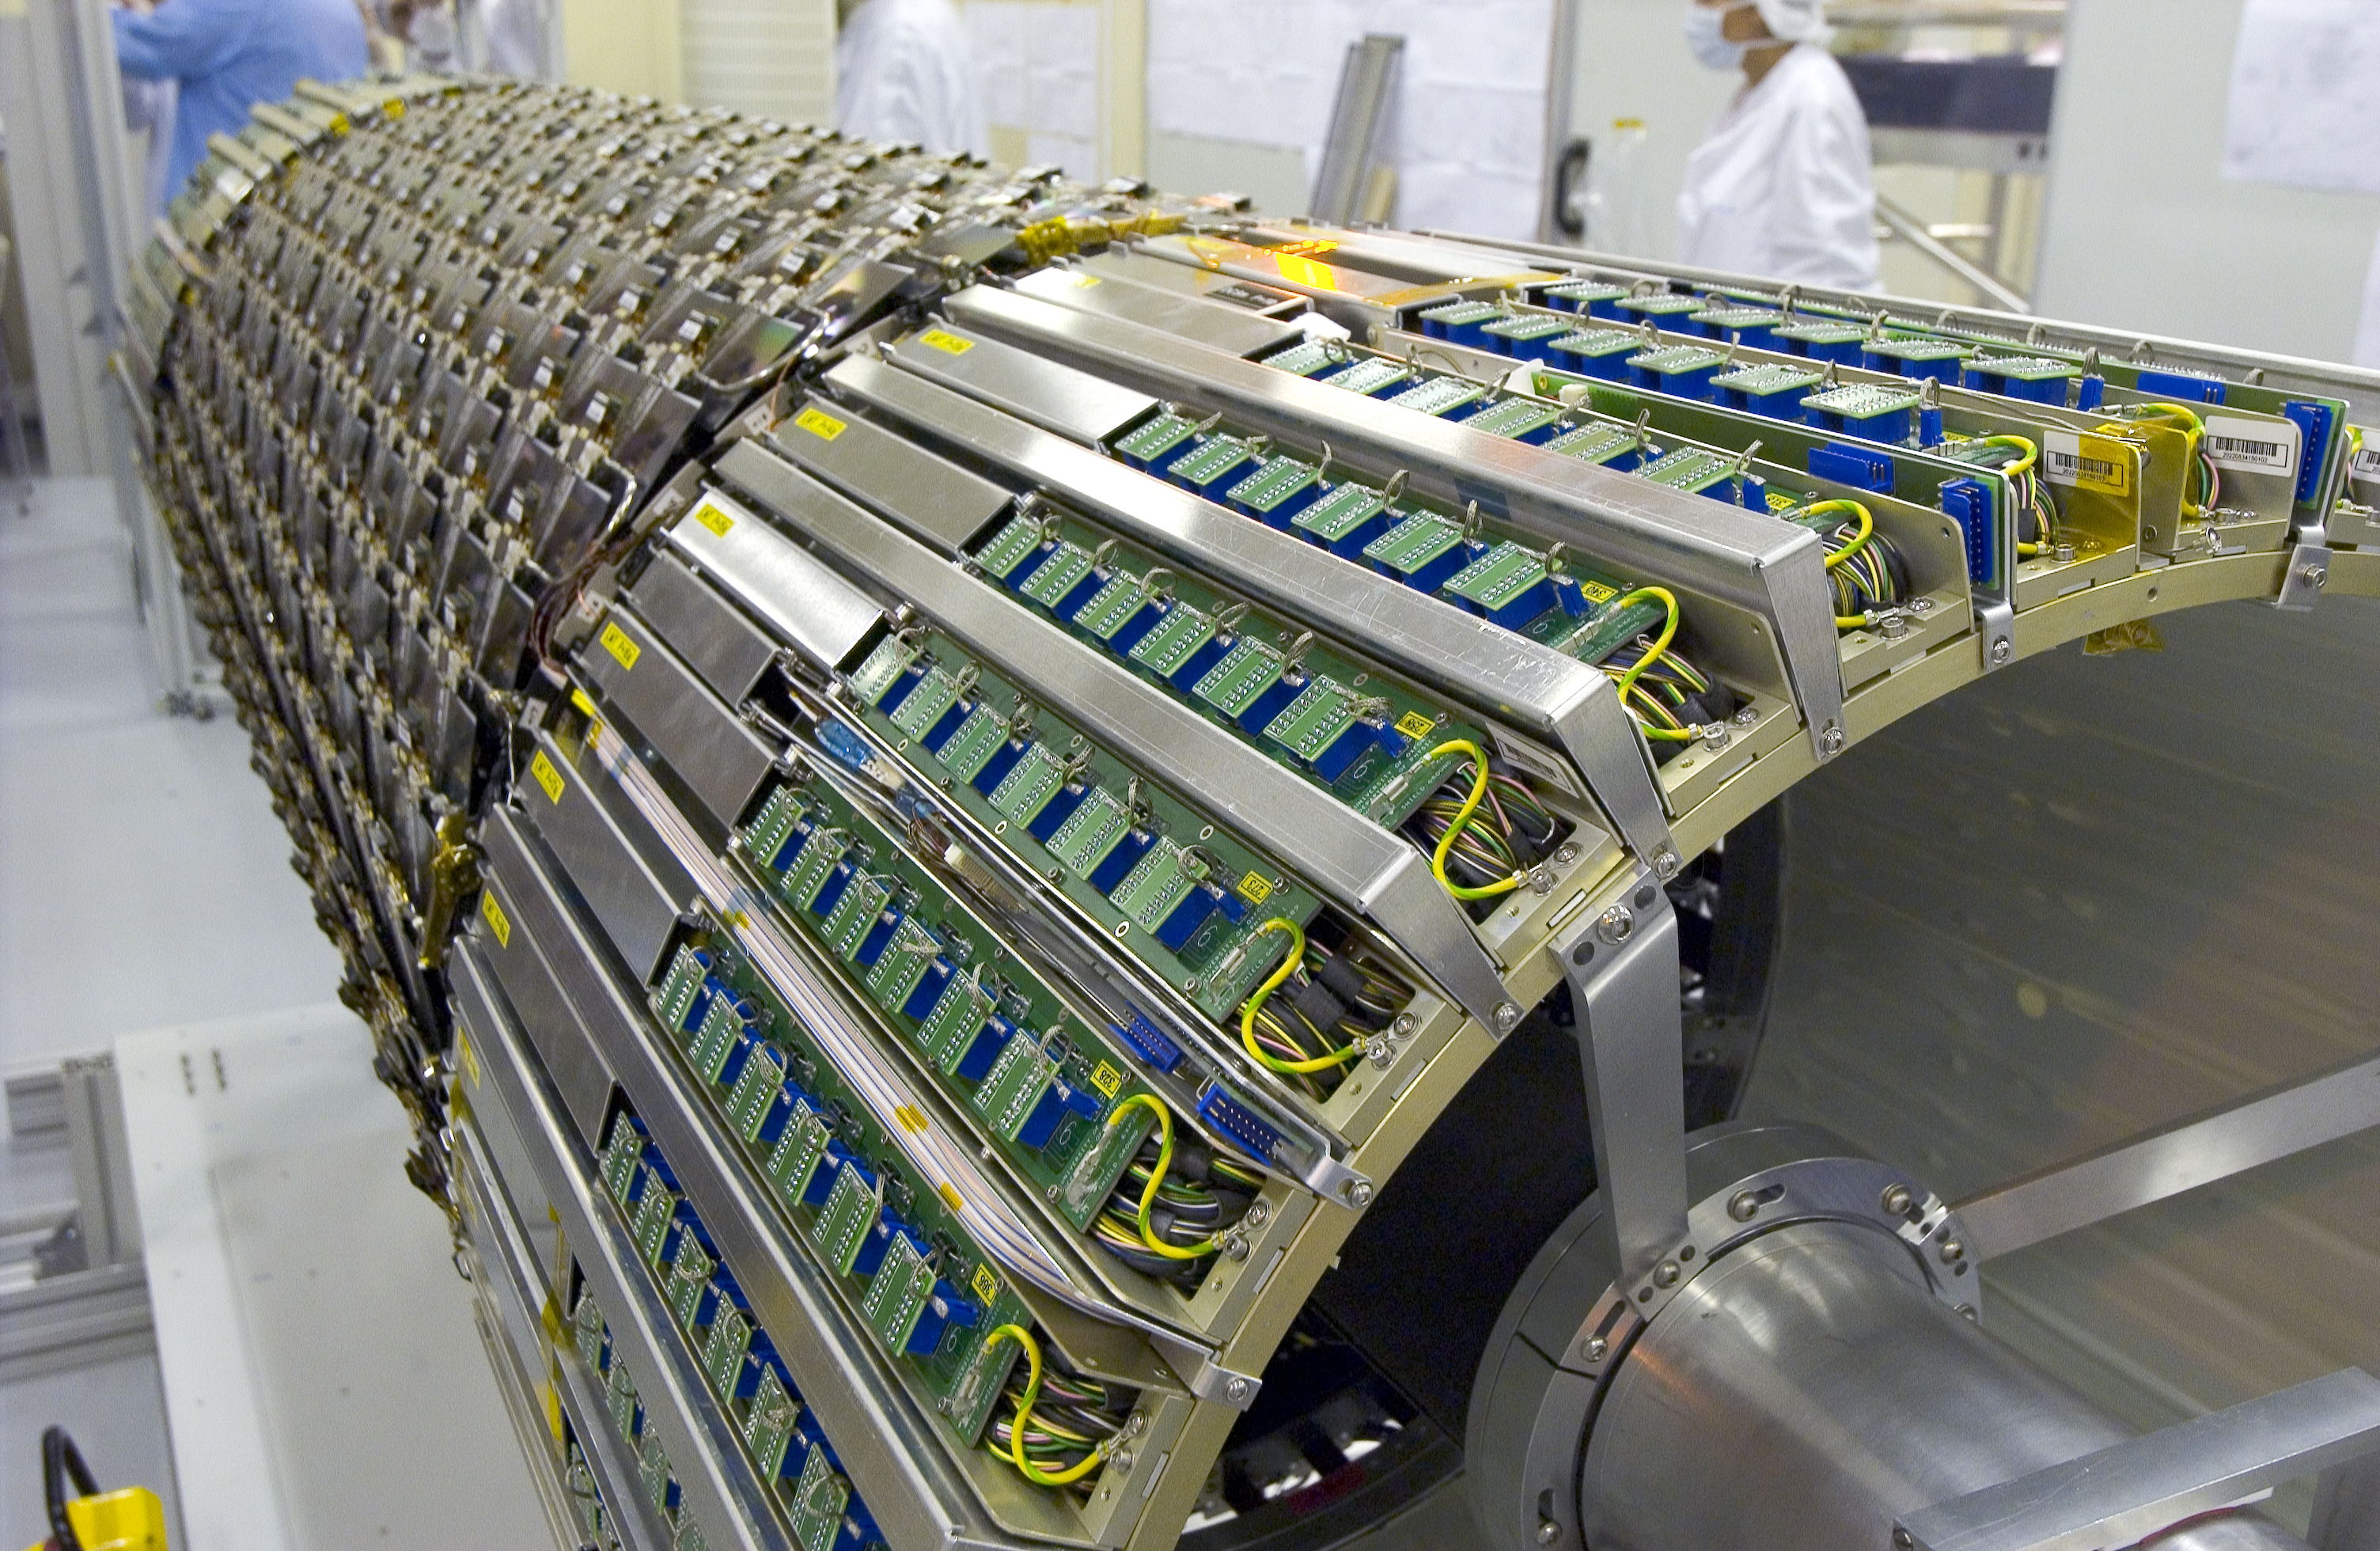
\includegraphics[width=\textwidth]{figs/lhc/sct_photo.jpg}
  }
  \caption{
    Photograph of the silicon semiconductor tracker of the
    \atlas\ experiment~\cite{Maximilien:883305}.
  }
  \label{fig:sct_photo}
\end{figure}

% \begin{figure}[ht]
%   \centering{
%     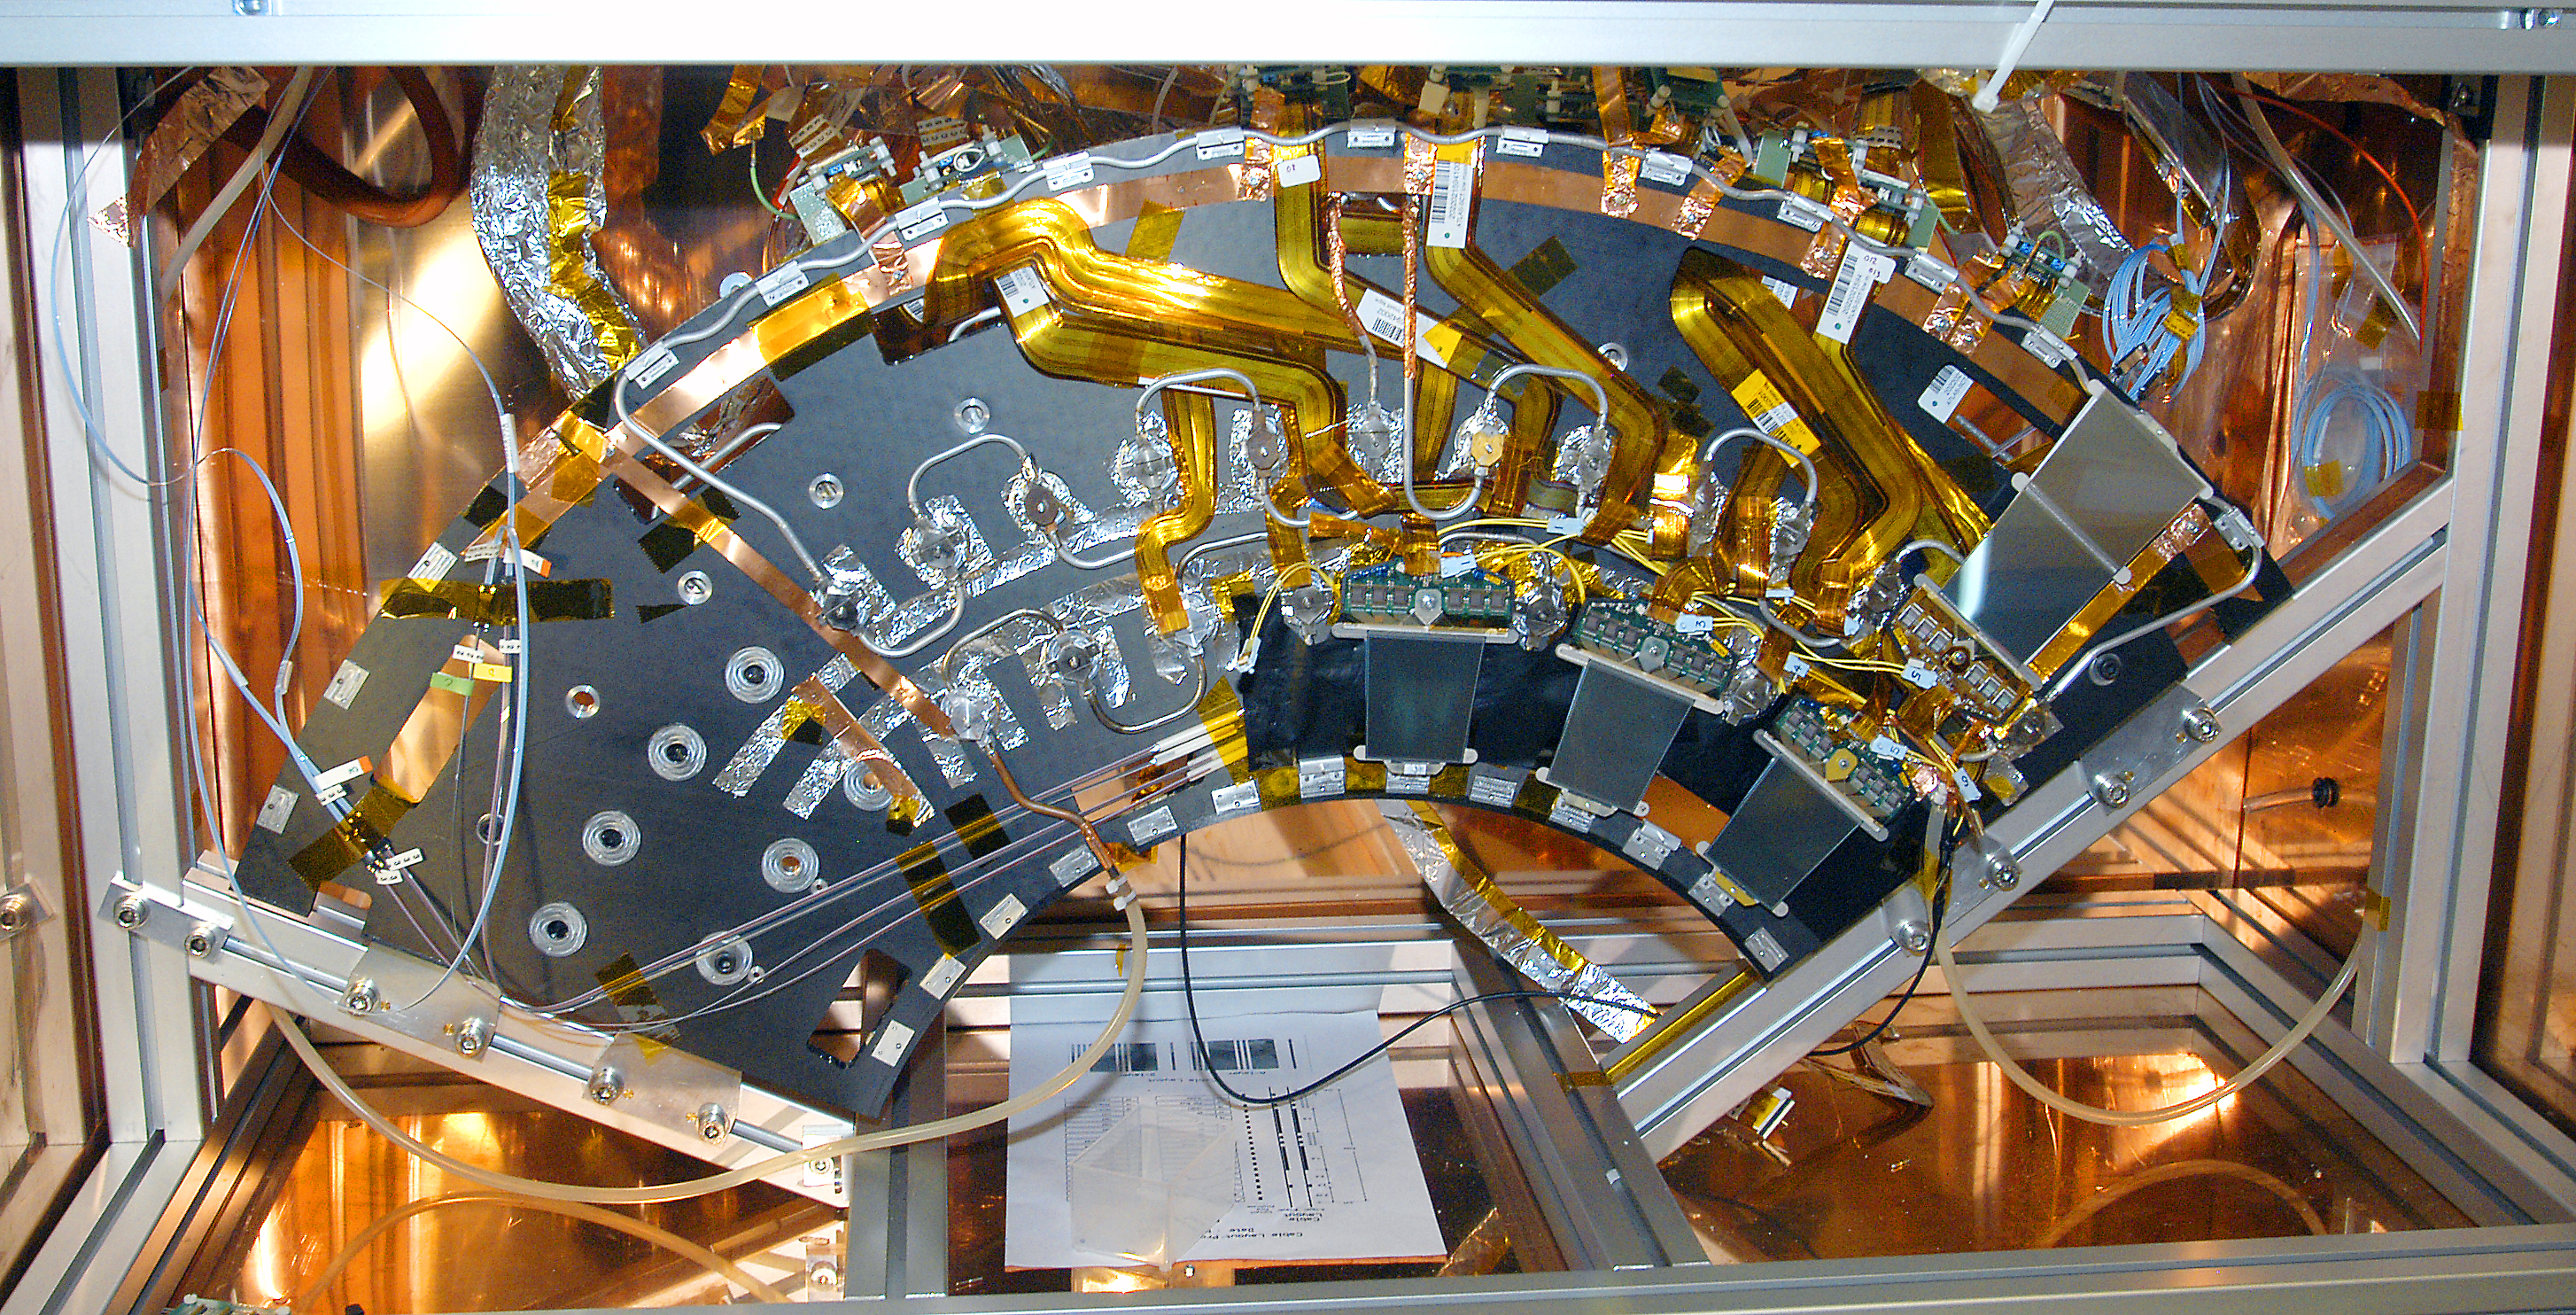
\includegraphics[width=0.8\textwidth]{figs/lhc/sct_close_up.jpg}
%   }
%   \caption{{\color{red}TODO}~\cite{Maximilien:43814}.}
%   \label{fig:sct_close_up}
% \end{figure}

%% - - - - - - - - - - - - - - - - - - - - - - - - - - - - - - - - - - - - - - -
\FloatBarrier
\subsubsection{Transition radiation tracker} 

{\color{red} Brief intro to TRT. }

{\color{red}This section should talk about how the TRT operates, going into
  what happens as a charged particle passes through the straw, and deposits
  charge, and ultimately creates a signal.
  % Then, I can get into $rt$ curves and tracking performance.
}

% {\color{red}I know less about this than TRT tracking, but since it's one of the
%   main functions of the TRT, I think it's important to at least discuss this
%     briefly}

\begin{figure}[ht]
  \centering{
    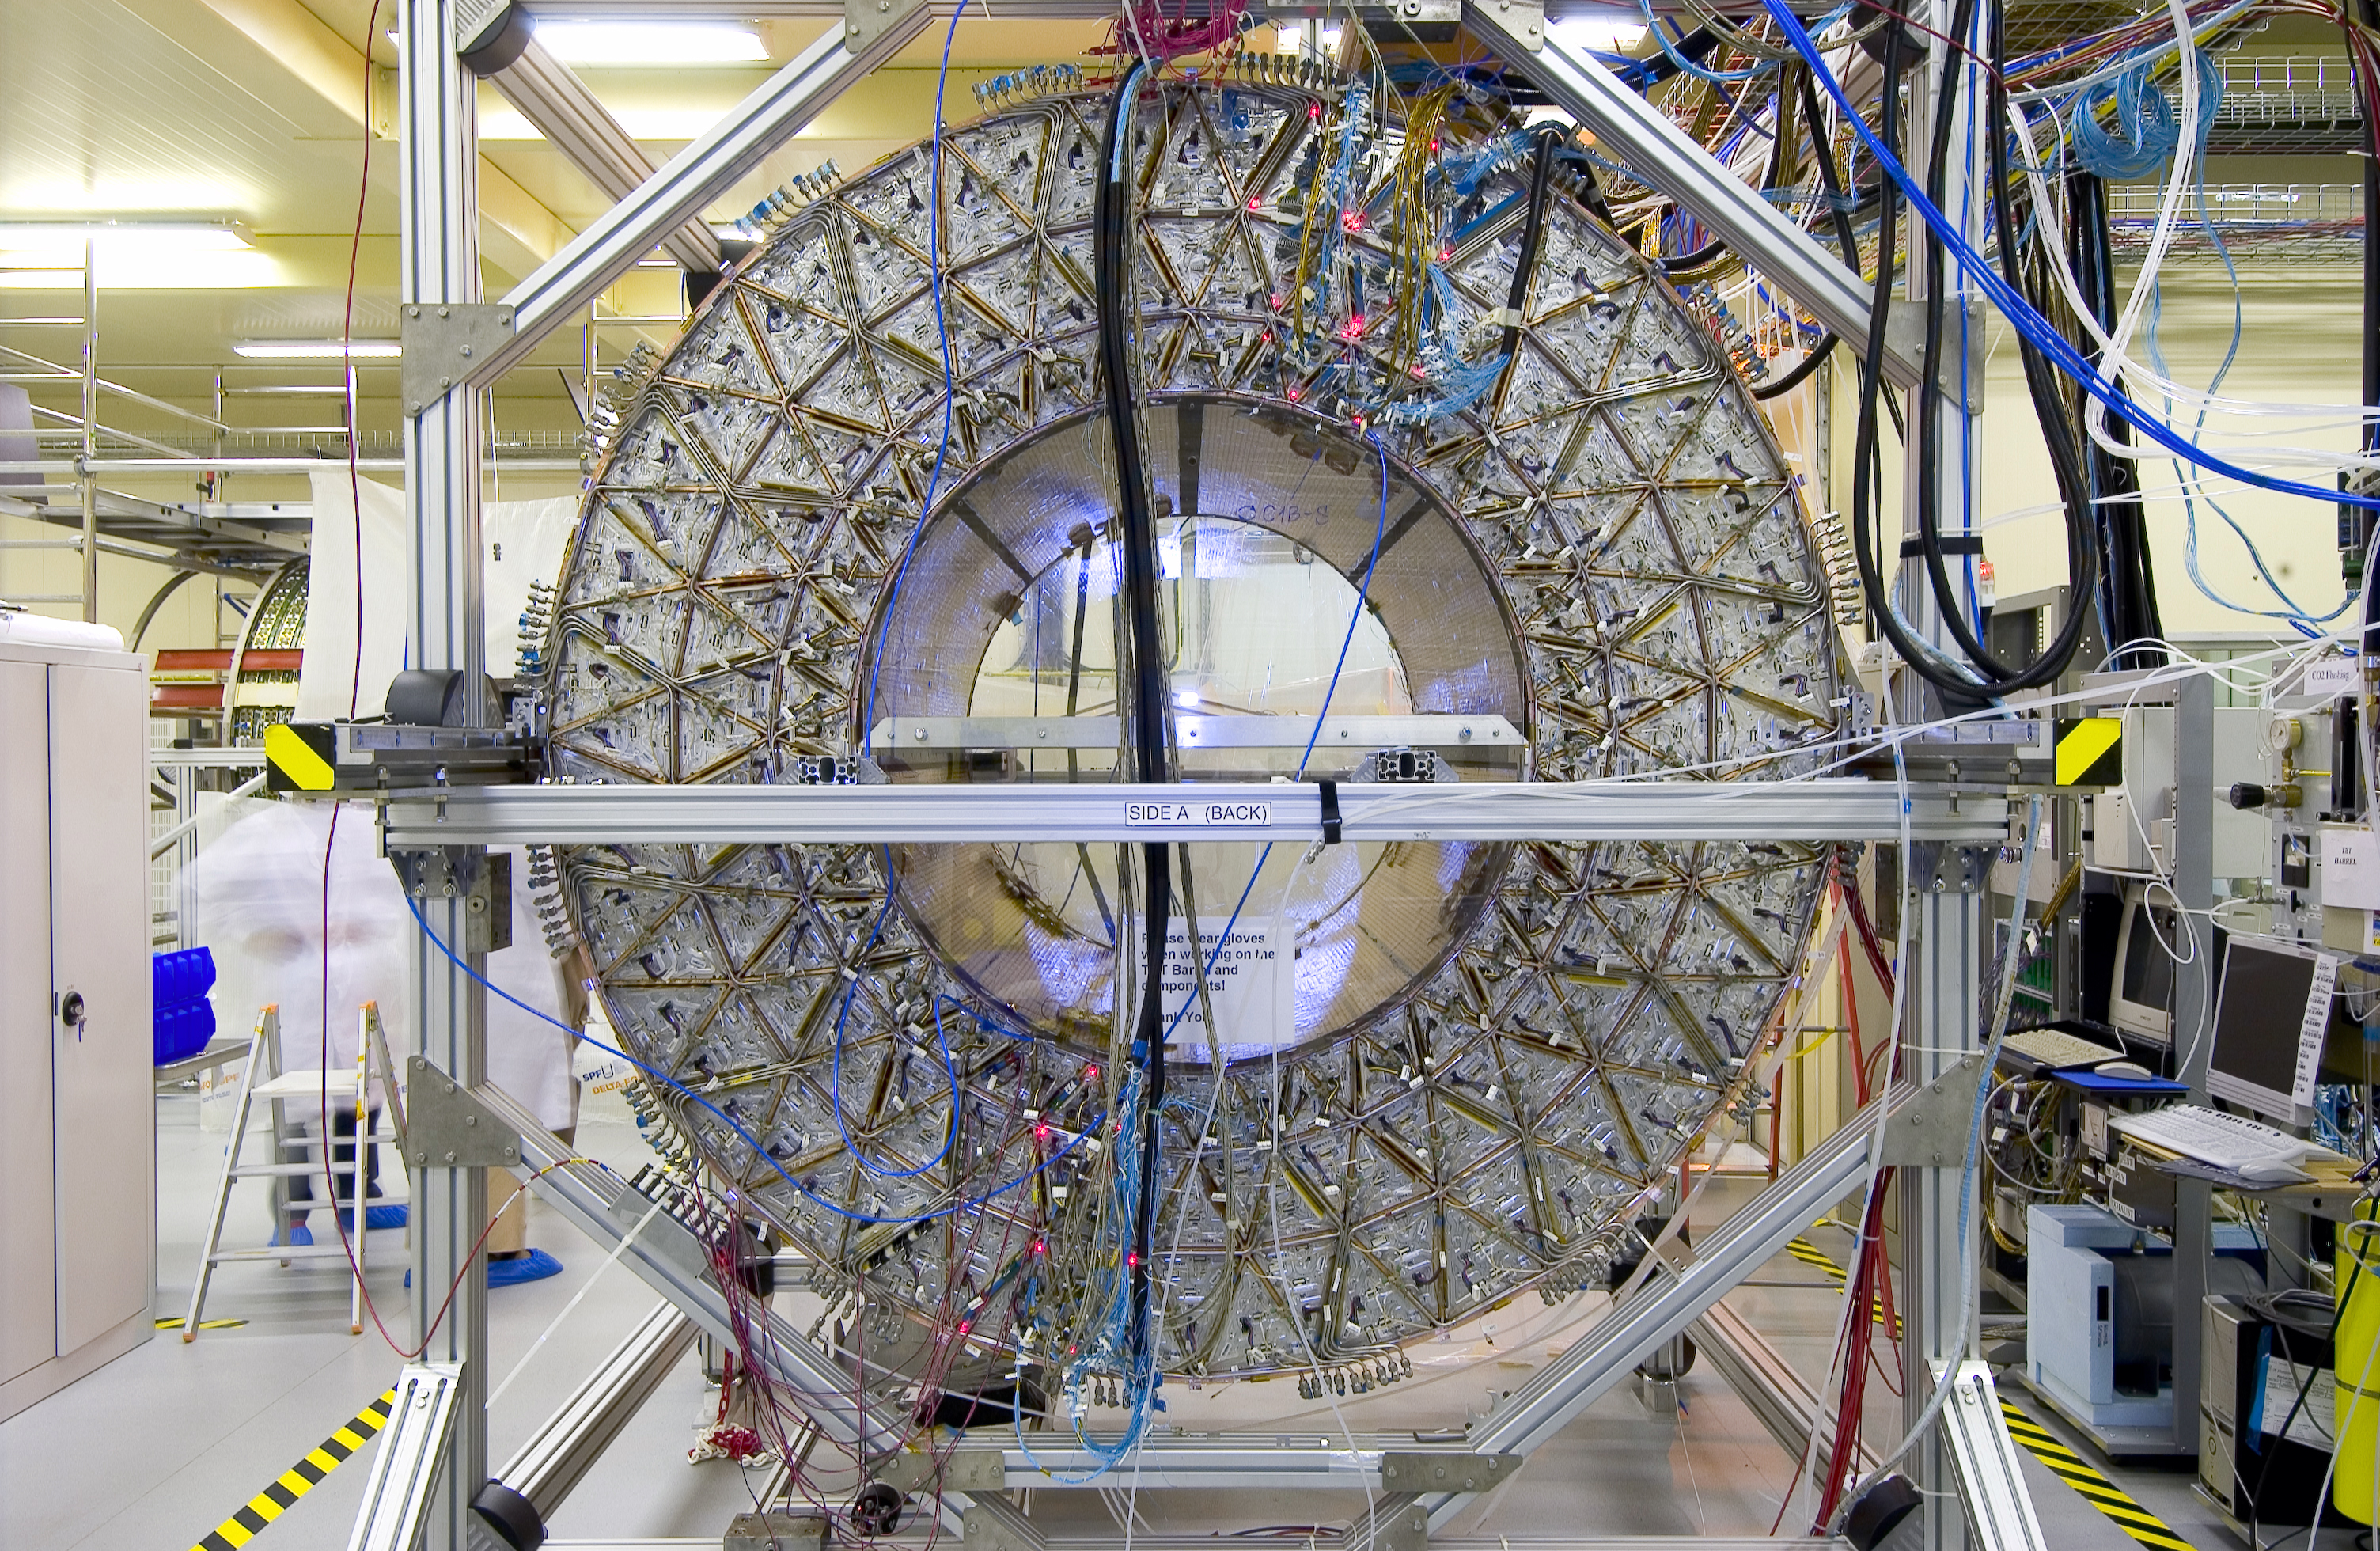
\includegraphics[width=\textwidth]{figs/lhc/trt_photo.jpg}
  }
  \caption{
    Photograph of the transition radiation tracker of the
    \atlas\ experiment during its commissioning~\cite{Maximilien:889555}.
  }
  \label{fig:trt_module}
\end{figure}

%% - - - - - - - - - - - - - - - - - - - - - - - - - - - - - - - - - - - - - - -
\FloatBarrier
\subsection{Calorimetry} 

{\color{red} Introduce the calo systems and its purpose}

\begin{figure}[ht]
  \centering{
    \includegraphics[width=\textwidth]{figs/lhc/calo_schematic.png}
  }
  \caption[
    Schematic of the calorimeter system of the
    \atlas\ experiment~\cite{cern-jinst-atlas}.
  ]{
    Schematic of the calorimeter system of the
    \atlas\ experiment.
    The calorimetry system is comprises the electromagnetic calorimeter,
    and a hadronic calorimeter~\cite{cern-jinst-atlas}.
  }
  \label{fig:calo_cartoon}
\end{figure}


%% - - - - - - - - - - - - - - - - - - - - - - - - - - - - - - - - - - - - - - -
\FloatBarrier
\subsubsection{Electromagnetic calorimeter} 

%% - - - - - - - - - - - - - - - - - - - - - - - - - - - - - - - - - - - - - - -
\FloatBarrier
\subsubsection{Hadronic calorimeter} 

%% - - - - - - - - - - - - - - - - - - - - - - - - - - - - - - - - - - - - - - -
\FloatBarrier
\subsection{Muon spectrometer} 

{\color{red} Introduce the MS and its purpose}

\begin{figure}[ht]
  \centering{
    \includegraphics[width=\textwidth]{figs/lhc/ms_schematic.jpg}
  }
  \caption{
    Schematic of the muon systems of the
    \atlas\ experiment~\cite{Pequenao:1095929}.
  }
  \label{fig:ms_cartoon}
\end{figure}


%% ------------------------------------------------------------------------------
\FloatBarrier
\section{Triggering system}

{\color{red} Why/how we trigger. What sort of rates we get. What is the
rejection rate at each trigger level...}

%% ------------------------------------------------------------------------------
\FloatBarrier
\section{Event reconstruction and object identification}
\label{sec:event_reco}

\begin{figure}[ht]
  \centering{
    \includegraphics[width=\textwidth]{figs/lhc/particle_signatures.jpg}
  }
  \caption{
    Schematic view of the signatures left in the various sub-detectors of
    \atlas\ in response to the primary particles which pass through
    it~\cite{Pequenao:1505342}.
  }
  \label{fig:particle_signatures}
\end{figure}

%% - - - - - - - - - - - - - - - - - - - - - - - - - - - - - - - - - - - - - - -
\FloatBarrier
\subsection{Electrons} 
\label{sec:elctrons}

{\color{red} TODO Write about electrons}

%% - - - - - - - - - - - - - - - - - - - - - - - - - - - - - - - - - - - - - - -
\FloatBarrier
\subsection{Muons} 
\label{sec:muons}

{\color{red} TODO Write about electrons}

%% - - - - - - - - - - - - - - - - - - - - - - - - - - - - - - - - - - - - - - -
\FloatBarrier
\subsection{Jets} 
\label{sec:jets}

{\color{red} TODO this is the text from the CONF note. Update and expand...}

Jets are reconstructed using the anti-$k_{t}$
algorithm~\cite{Cacciari:2008gp, Cacciari:2005hq} with a radius
parameter $R = $ 0.4 from calibrated clusters of energy deposits in
the calorimeters. The differences in calorimeter response between
electrons, photons and hadrons are taken into account by classifying
each cluster, prior to the jet reconstruction, as coming from an
electromagnetic or hadronic shower on the basis of its shape
\cite{JES}.  The jet energy thus accounts for electromagnetic
and hadronic energy deposits at the cluster level with correction
factors derived from MC simulation.  A further correction,
used to calibrate the jet energy to the scale of its constituent
particles, (JES) \cite{JES,JES2}, is then applied.  The impact of
pileup is accounted for using
a technique, based on jet areas, that provides an event-by-event and
jet-by-jet correction \cite{Cacciari:2007fd}.  Jets are required
to have transverse momentum \pt\ $>$ 40~\GeV\ and $|\eta| < 4.9$.
In order to reduce contamination from jets produced by pileup,
the scalar sum of the \pt\ of the tracks matched to the jet and
originating from the primary vertex must be at least 50\% of the
scalar sum of the \pt\ of all tracks matched to the jet.  This
criterion is only applied to jets with $\pt < 50 \GeV$ and $|\eta| < 2.4$.

%% - - - - - - - - - - - - - - - - - - - - - - - - - - - - - - - - - - - - - - -
\FloatBarrier
\subsection{Flavor tagging} 
\label{sec:flavor_tagging}

{\color{red} TODO this is the text from the CONF note. Update and expand...}

The identification of $b$-jets uses the MV1 flavor tagging
algorithm~\cite{ATLAS-CONF-2014-004, ATLAS-CONF-2014-046}, which is
based on an artificial neural network
algorithm that exploits the impact parameters of charged particle
tracks, the parameters of reconstructed secondary vertices, and the
topology of $b$- and $c$-hadron decays inside a jet.  The operating
point corresponds to an overall 80\% $b$-tagging efficiency, as
measured in simulated \TTBAR\ events, a rejection factor of 25 for jets
originating from light quarks or gluons, and a rejection factor of
3 for jets originating from charm quarks.

%% - - - - - - - - - - - - - - - - - - - - - - - - - - - - - - - - - - - - - - -
\FloatBarrier
\subsection{Missing energy} 
\label{sec:met}

% {\color{red} missing momentum?}
{\color{red} TODO this is the text from the CONF note. Update and expand...}

The vector momentum imbalance in the transverse plane is obtained from
the negative vector sum of the reconstructed and calibrated physics
objects and the calorimeter energy clusters not associated with reconstructed
objects. This is denoted as missing transverse momentum, and the symbol
$\met$ is used for its magnitude.  The $\met$ calculation is described
elsewhere~\cite{ATLAS-CONF-2013-082}.
